
The results were obtained using the
PDF4LHC15{\tt\_}nlo{\tt\_}30{\tt\_}pdfas~\cite{Butterworth:2015oua,CT14,MMHT14,NNPDF}
parton distribution functions interfaced to our code via
LHAPDF~\cite{Buckley:2014ana}, along with the corresponding value for
$\alpha_s$.  The masses of the Higgs boson and the top quark have been
fixed, as in the virtual amplitude, to $m_h=125$\,GeV, $m_t=173$\,GeV,
respectively. Their widths have been set to zero.   
Jets are clustered with the
anti-$k_T$ algorithm~\cite{Cacciari:2008gp} as implemented in the
{\tt fastjet} package~\cite{Cacciari:2005hq, Cacciari:2011ma}, with jet
radius $R=0.4$ and a minimum transverse momentum 
$p_{T,\mathrm{min}}^{\rm{jet}}=20$\,GeV.  The scale uncertainties are
estimated by varying the factorisation/renormalisation scales
$\mu_{F}, \mu_{R}$. The scale variation bands 
represent scale variations around the central scale $\mu_0 =\mhh/2$, with
$\mu_{R} = \mu_{F}=c\,\mu_0$, where $c \in \{0.5,1,2\}$.
For the case $\lambda=\lambda_{\mathrm{SM}}$ we checked that the bands
obtained from these variations coincide with the bands resulting from
7-point scale variations. The PDF uncertainties have been studied in
\cite{deFlorian:2016spz} and found to be in general considerably smaller than the scale uncertainties.

\subsection{Total cross sections at different values of the trilinear coupling}

In Table \ref{tab:sigmatot} we list total cross sections at 13, 14 and 27\,TeV for various values of the trilinear Higgs coupling $\lambda$. 
\begin{table}[htb]
\begin{center}
%\setlength{\extrarowheight}{3.0pt}
\begin{tabular}{| c | c | c |c|c|}
%\Xhline{2\arrayrulewidth}
\hline
&&&&\\
$\lambda_{\mathrm{BSM}}/\lambda_{\mathrm{SM}}$ & $\sigma_{\rm{NLO}}@13 \mathrm{TeV}$\,[fb]& $\sigma_{\rm{NLO}}@14 \mathrm{TeV}$\,[fb] & $\sigma_{\rm{NLO}}@27 \mathrm{TeV}$\,[fb] &K-factor@14TeV\\
&&&&\\
\hline
-1& 116.71$^{+16.4\%}_{-14.3\%}$  & 136.91$^{+16.4\%}_{-13.9\%}$& 504.9 & 1.86 \\
\hline
0& 62.51$^{+15.8\%}_{-13.7\%}$ & 73.64$^{+15.4\%}_{-13.4\%}$& 275.29& 1.79  \\
\hline 
1& 27.84$^{+11.6\%}_{-12.9\%}$ & 32.88$^{+13.5\%}_{-12.5\%}$&127.7$^{+11.5\%}_{-10.4\%}$ &1.66\\
\hline
2 & 12.42$^{+13.1\%}_{-12.0\%}$ & 14.75$^{+12.0\%}_{-11.8\%}$ &  59.10 & 1.56 \\
\hline
2.4& 11.65$^{+13.9\%}_{-12.7\%}$ & 13.79$^{+13.5\%}_{-12.5\%}$& 53.67 & 1.65 \\
\hline
3& 16.28$^{+16.2\%}_{-15.3\%}$ & 19.07$^{+17.1\%}_{-14.1\%}$ & 69.84 & 1.90 \\
\hline 
5& 81.74$^{+20.0\%}_{-15.6\%}$  & 95.22$^{+19.7\%}_{-11.5\%}$& 330.61 & 2.14 \\
\hline 
\end{tabular}
\end{center}
\caption{Total cross sections for Higgs boson pair production at full NLO QCD. The given uncertainties are scale uncertainties. 
\label{tab:sigmatot}}
\end{table}
Table~\ref{tab:sigmatot} also shows that the K-factors vary substantially as functions of the trilinear coupling.
This fact is illustrated in Fig.~\ref{fig:Kfacvariation}, showing that the K-factor takes values between 1.56 and 2.14
if the trilinear coupling is varied between $-5\leq \chhh\leq 12$.

\begin{figure}[htb]
  \centering
    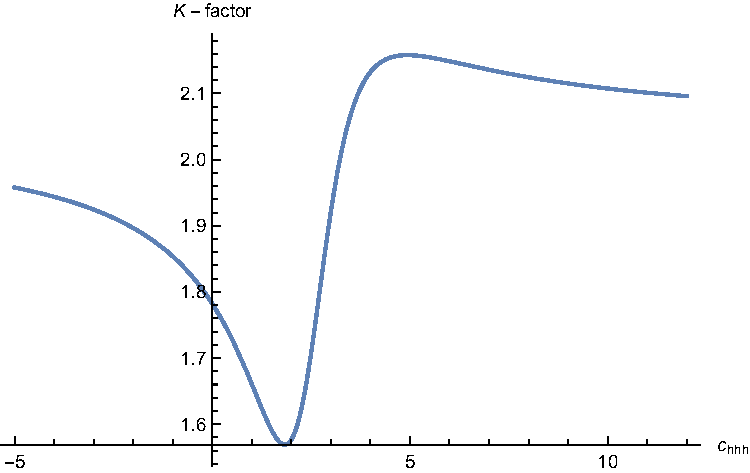
\includegraphics[width=0.45\textwidth]{plots/Kfac_varlambda.pdf}
%  \includegraphics[width=\textwidth]{plots/}
%    \caption{\label{fig:lambda_large_27}}
\caption{Variation of the NLO K-factor with the trilinear coupling at $\sqrt{s}=14$\,TeV.}
\label{fig:Kfacvariation}
\end{figure}


\subsection{Differential cross sections}

In Fig.~\ref{fig:lambdavar14TeV} we show the $\mhh$ distribution for various values of $\chhh=\lambda_{\mathrm{BSM}}/\lambda_{\mathrm{SM}}$. 
The ratio plots show the ratio to the result with $\lambda_{\mathrm{SM}}$. 
A characteristic dip develops in the $\mhh$ distribution around $\chhh=2.4$, which is the value of maximal destructive interference between diagrams containing the trilinear coupling (triangle-type contributions) and ``background" diagrams (box-type contributions).
Therefore we provide results for a denser spacing of $\chhh$ values around this point.

\begin{figure}[htb]
 \begin{subfigure}[t]{0.495\textwidth}
\includegraphics[width=\textwidth]{plots/{NLO_cHHH_1_2_2.4_0_mHH-paper}.pdf}
%    \vspace{\TwoFigBottom em}
\caption{\label{fig:lambda_small}}
\end{subfigure}
\hfill
\begin{subfigure}[t]{0.495\textwidth}
    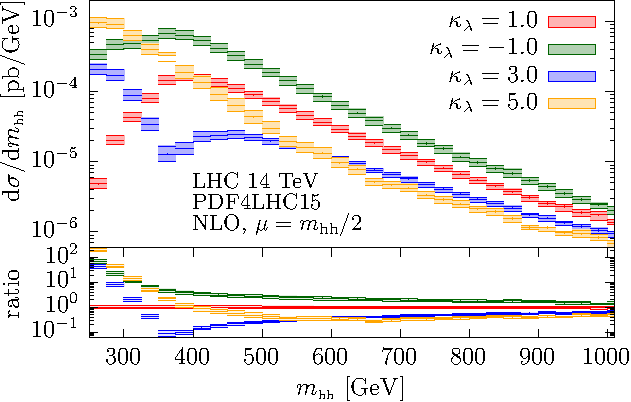
\includegraphics[width=\textwidth]{plots/NLO_cHHH_1_-1_3_5_mHH-paper.pdf}
\caption{\label{fig:lambda_large}}
\end{subfigure}
\caption{Higgs boson pair invariant mass distributions for various
  values of $\chhh$  at $\sqrt{s}=14$\,TeV. The uncertainty bands are from
  scale variations as described in the text.}
\label{fig:lambdavar14TeV}
\end{figure}

\begin{figure}[htb]
 \begin{subfigure}[t]{0.495\textwidth}
\includegraphics[width=\textwidth]{plots/{NLO_cHHH_1_2_2.4_0_ptH-a}.pdf}
\caption{\label{fig:lambda_small_pTH}}
\end{subfigure}
\hfill
\begin{subfigure}[t]{0.495\textwidth}
    \includegraphics[width=\textwidth]{plots/{NLO_cHHH_1_-1_3_5_ptH-a}.pdf}
\caption{\label{fig:lambda_large_pTH}}
\end{subfigure}
\caption{Higgs boson transverse momentum distributions for various values of $\chhh$  at $\sqrt{s}=14$\,TeV.
\label{fig:lambdavar14TeV_pTH}}
\end{figure}
In Fig.~\ref{fig:lambdavar14TeV_pTH} we show the transverse momentum
distributions $p_T^h$ of one (any) Higgs boson for different $\chhh$
values. The dip for $\chhh\sim 2.4$ is still present, however much
less pronounced than in the $\mhh$ distribution.

\begin{figure}[htb]
 \begin{subfigure}[t]{0.495\textwidth}
\includegraphics[width=\textwidth]{plots/{NLO_CPP_yt_0.8_1.2_mHH}.pdf}
\caption{\label{fig:ytvar_mhh}}
\end{subfigure}
\hfill
\begin{subfigure}[t]{0.495\textwidth}
\includegraphics[width=\textwidth]{plots/{NLO_CPP_yt_0.8_1.2_pTH-a}.pdf}
\caption{\label{fig:ytvar_pth}}
\end{subfigure}
\caption{Higgs boson pair invariant mass distributions, and distributions of the transverse momentum of one (any) Higgs boson for non-SM values of the top quark Yukawa coupling $y_t$  at $\sqrt{s}=14$\,TeV, including scale uncertainties.
\label{fig:ytvar}}
\end{figure}

Fig.~\ref{fig:ytvar} demonstrates the effect of variations of the top quark Yukawa coupling $y_t$ on the $\mhh$ and $\pth$ distributions, where $\chhh$ is fixed to the SM value.
Using eq.~(\ref{eq:yt}), it is apparent that $y_t$ variations can be obtained from appropriate $\chhh$ variations with the same code.
For example, $\sigma(y_t=1.2,\chhh=1)=(1.2)^4\,\sigma(y_t=1,\chhh=1/1.2)$.

\subsection{Discussion of parton shower related uncertainties} 
 
In this section we show distributions for NLO results matched to a
parton shower, focusing mostly on the transverse momentum of the Higgs
boson pair. For this distribution 
NLO is the first non-trivial order, and therefore it is particularly
sensitive to differences in the treatment of radiation by the
parton shower.
We compare the \pythia~\cite{Sjostrand:2014zea} and \herwig~\cite{Bellm:2017bvx} parton showers, 
applied directly to the \powheg{} Les Houches events (LHE).
In the \herw case, we also compare the default shower (the angular-ordered $\tilde{q}$-shower) 
with the dipole shower.
In addition, we assess the uncertainties stemming from the matching and show results where the 
\herw shower scale parameter {\tt HardScale} is varied. For all shower algorithms considered, the default 
tune of the corresponding version is used. Multiple-parton interactions (MPI) and hadronisation 
are switched off. The \hdamp{} parameter in \powheg{} is set to $\hdamp=250$\,GeV.

\begin{figure}[htb]
 \begin{subfigure}[t]{0.495\textwidth}
\includegraphics[width=\textwidth]{plots/{NLO_PP8_PH7_PH7D_cHHH_1_ptH-a}.pdf}
 \caption{\label{fig:lambda_pTh}}
\end{subfigure}
\hfill
\begin{subfigure}[t]{0.495\textwidth}
    \includegraphics[width=\textwidth]{plots/{NLO_PP8_PH7_PH7D_cHHH_1_dRHH}.pdf}
\caption{\label{fig:lambda_dRHH}}
\end{subfigure}
\caption{The transverse momentum of one (any) Higgs boson and the $R$-separation between 
the two Higgs bosons are shown for the fixed-order NLO calculation and three shower setups, in 
the $\chhh=1$ case.
\label{fig:lambdavar14TeV_pTH_dRHH_showers}}
\end{figure}

In general, observables that are inclusive in the additional radiation, like the 
transverse momentum of one (any) Higgs boson, $p_T^h$, show little sensitivity to the details of 
the parton showering, as highlighted in Fig.~\ref{fig:lambda_pTh} for the fixed-order NLO prediction, 
as well as for the \pythia (PP8) and both \herwig showers (angular-ordered PH7-$\tilde{q}$, 
and PH7-dipole). In contrast, Fig.~\ref{fig:lambda_dRHH} 
shows the distribution of the distance $\Delta
R^{\mathrm{hh}}=\sqrt{(\eta_1-\eta_2)^2+(\Phi_1-\Phi_2)^2}$ between the two Higgs 
bosons. There, the Sudakov exponent and the parton shower effectively resum the fixed-order 
prediction in the region where the two Higgs bosons are close to a back-to-back configuration, 
and the parton shower increases the fixed-order real radiation contribution in the region $\Delta R^{\mathrm{hh}}<\pi$.

\begin{figure}[htb]
 \begin{subfigure}[t]{0.495\textwidth}
\includegraphics[width=\textwidth]{plots/{NLO_PP8_PH7_PH7D_cHHH_1_ptHH}.pdf}
 \caption{\label{fig:lambda_ptHH_cHHH1}}
\end{subfigure}
\hfill
\begin{subfigure}[t]{0.495\textwidth}
    \includegraphics[width=\textwidth]{plots/{NLO_PP8_PH7_PH7D_cHHH_2.4_ptHH}.pdf}
\caption{\label{fig:lambda_ptHH_cHHH2.4}}
\end{subfigure}
\caption{Transverse momentum of the Higgs boson pair for the fixed-order NLO calculation 
and all three shower setups at 14\,TeV for (a) $\chhh=1$, (b) $\chhh=2.4$.
\label{fig:lambdavar14TeV_pTHH_showers}}
\end{figure}

In Figs.~\ref{fig:lambda_ptHH_cHHH1} and \ref{fig:lambda_ptHH_cHHH2.4}, the transverse 
momentum $\pthh$ of the Higgs boson pair system is shown for the same fixed-order and parton-showered predictions, at $\chhh=1$ and $\chhh=2.4$. In all cases, the \pyth and \herw showers 
agree very well in the small-$\pthh$ range, but start to deviate already at $\pthh \sim 100$\,GeV. 
While both \herw showers give very similar results and reproduce the fixed-order calculation at high-$\pthh$, the 
\pyth shower produces much harder additional radiation and the ratio to the fixed-order result stagnates at $\sim 2.0$ over the remaining range. 
%A discussion of the surprisingly hard tail of the $\pthh$ distribution with \powheg+\pythia can be found in
%Refs.~\cite{Jones:2017giv,Bendavid:2018nar}, where the results are also
%compared to two different showers within {\sc Sherpa}~\cite{Gleisberg:2008ta,Schumann:2007mg,Hoche:2015sya} as well
%as with {\sc MG5\_aMC@NLO}~\cite{Alwall:2014hca,Hirschi:2015iia}.
We should also mention that rather large differences between \pythia and
\herwig showers matched to \powheg{} also have been found studying top
quark pair production~\cite{Ravasio:2018lzi}. The origin of the large NLO parton shower matching uncertainties affecting certain observables in Higgs boson pair production have previously been studied in literature~\cite{Jones:2017giv}. For the SM result, the excess at large $\pthh$ produced when using \powheg{} with \pythia was found to be due to additional hard sub-leading jets generated purely by the shower~\cite{Bendavid:2018nar}.

With the \herw default shower, systematic uncertainties can be estimated by 
varying the maximal transverse momentum allowed for shower emissions,
by changing the so-called hard scale $\mu_Q$. We apply a factor $c_Q=\{0.5,\,2.0\}$ on the central hard shower scale, separately 
for all variations of the factorisation/renormalisation scales
$\mu_{R,F}$.
%, which is the standard use in the \herw setup. 
Fig.~\ref{fig:lambdavar14TeV_muQvar} shows the $\pthh$ and 
$\Delta R^{\mathrm{hh}}$ distributions as examples of the SM case, $\chhh=1$, and underlines 
their sensitivity to changes in the shower hard scale. Quantitatively, the hard scale variations 
inflate the sole factorisation/renormalisation scale uncertainties by a factor of two in 
the regions where the \herwig and \pythia showers were in disagreement (see Figs.~\ref{fig:lambda_dRHH} 
and \ref{fig:lambdavar14TeV_pTHH_showers}). If the envelope of all scale variations, including 
the hard shower scale, was to be taken as a theoretical systematic uncertainty, the resulting 
uncertainty would be of the order of 50\% in these bins. It would be enlightening to further study 
parton-shower (and non-perturbative) effects, in the particular context of Higgs boson pair 
production at NLO, as well as for loop-induced colour singlet production in general, and try to reduce discrepancies among the different algorithms. 


\begin{figure}[htb]
 \begin{subfigure}[t]{0.495\textwidth}
\includegraphics[width=\textwidth]{plots/{PP8_PH7_PH7QUp_PH7QDown_cHHH_1_ptHH}.pdf}
 \caption{\label{fig:lambda_ptHH_muQvar}}
\end{subfigure}
\hfill
\begin{subfigure}[t]{0.495\textwidth}
    \includegraphics[width=\textwidth]{plots/{PP8_PH7_PH7QUp_PH7QDown_cHHH_1_dRHH}.pdf}
\caption{\label{fig:lambda_dRHH_muQvar}}\end{subfigure}
\caption{Higgs boson pair transverse momentum and $R$-separation for variations of the \herw $\tilde{q}$-shower hard scale.
\label{fig:lambdavar14TeV_muQvar}}
\end{figure}
